% ================================================
% ADVANCED EXAMPLE - Hebrew Academic Template
% ================================================
% This example demonstrates advanced features including bibliography,
% complex tables, multiple code examples, and cross-references
% Compiles to approximately 10-12 pages
% Copyright (c) 2025 Dr. Segal Yoram. All rights reserved.

\documentclass{hebrew-academic-template}

% Force figure/table positioning
\usepackage{float}

% Add bibliography file
\addbibresource{advanced_references.bib}

% Title page information
\hebrewtitle{דוגמה מתקדמת - תבנית אקדמית עברית}
\englishtitle{Advanced Example - Hebrew Academic Template \clsversion}
\hebrewauthor{ד"ר סגל יורם}
\hebrewversion{גרסה \en{\clsversion}}
\date{\textenglish{January 2026}}

\begin{document}

\maketitle
\tableofcontents
\listoffigures
\listoftables
\newpage

% ==================== ADVANCED INTRODUCTION ====================

\hebrewsection{מבוא מתקדם: \entoc{Advanced Introduction}}

מסמך זה מדגים יכולות מתקדמות של התבנית האקדמית העברית גרסה \en{\clsversion},
כולל שימוש בביבליוגרפיה מתקדמת, טבלאות מורכבות, ודוגמאות קוד מרובות.

\hebrewsubsection{סקירת ספרות מקיפה: \entoc{Comprehensive Literature Review}}

המחקר בתחום \en{Natural Language Processing} עבר מהפכה עם הצגת ארכיטקטורת \en{Transformer} \cite{vaswani2017attention}.
מודל \en{BERT} \cite{devlin2018bert} הביא לפריצת דרך בהבנת שפה דו-כיוונית.
מחקרים בעברית \cite{hebrew_nlp_2023,hebrew_linguistics_2022} מראים התקדמות משמעותית.

עבודות נוספות \cite[עמ' 15-20]{bert_paper_2018} מדגימות שיפור של \percent{25.8} בביצועים.
המחקר של \cite[פרק 3]{gpt3_paper_2020} מציג ארכיטקטורה עם \num{175e9} פרמטרים.

% ==================== COMPLEX TABLES ====================

\hebrewsection{טבלאות מורכבות ומתקדמות: \entoc{Complex and Advanced Tables}}

\hebrewsubsection{טבלת ביצועים מפורטת: \entoc{Detailed Performance Table}}

\begin{table}[H]
\caption{ביצועי מודלים על מטלות שונות: \entoc{Model Performance on Various Tasks}}
\label{tab:performance}
\centering
\resizebox{\textwidth}{!}{%
\begin{tblr}{
  colspec = {cccccc},
  row{1} = {font=\bfseries, bg=blue9, fg=white},
  row{even} = {bg=gray9},
  hlines,
  vlines,
}
מודל / \en{Model} & סיווג / \en{Classification} & תרגום / \en{Translation} & סיכום / \en{Summarization} & מענה / \en{QA} & ממוצע / \en{Average} \\
\en{BERT-Base} & \percent{92.3} & \en{N/A} & \percent{85.2} & \percent{88.9} & \percent{88.8} \\
\en{BERT-Large} & \percent{94.1} & \en{N/A} & \percent{87.5} & \percent{91.2} & \percent{90.9} \\
\en{GPT-2} & \percent{89.7} & \percent{82.3} & \percent{88.1} & \percent{85.4} & \percent{86.4} \\
\en{GPT-3} & \percent{95.2} & \percent{91.7} & \percent{92.3} & \percent{93.8} & \percent{93.3} \\
\en{T5-Base} & \percent{93.5} & \percent{89.2} & \percent{90.1} & \percent{90.7} & \percent{90.9} \\
\en{T5-Large} & \percent{95.8} & \percent{92.4} & \percent{93.2} & \percent{94.1} & \percent{93.9} \\
מודל עברי / \en{HeBERT} & \percent{89.3} & \percent{78.5} & \percent{81.2} & \percent{86.7} & \percent{83.9} \\
\end{tblr}%
}
\end{table}

כפי שניתן לראות בטבלה \ref{tab:performance}, המודלים הגדולים משיגים ביצועים טובים יותר.

\hebrewsubsection{טבלת השוואת משאבים: \entoc{Resource Comparison Table}}

\begin{table}[H]
\caption{דרישות משאבי חישוב: \entoc{Computational Resource Requirements}}
\label{tab:resources}
\centering
\resizebox{\textwidth}{!}{%
\begin{tblr}{
  colspec = {ccccc},
  row{1} = {font=\bfseries, bg=blue9, fg=white},
  row{even} = {bg=gray9},
  hlines,
  vlines,
}
מודל / \en{Model} & פרמטרים / \en{Parameters} & זיכרון / \en{Memory} & זמן אימון / \en{Training Time} & עלות / \en{Cost} \\
\en{BERT-Base} & \num{110e6} & \en{440 MB} & \num{4} ימים & \en{\$}\num{500} \\
\en{BERT-Large} & \num{340e6} & \en{1.3 GB} & \num{12} ימים & \en{\$}\num{2000} \\
\en{GPT-2 Medium} & \num{345e6} & \en{1.4 GB} & \num{7} ימים & \en{\$}\num{1500} \\
\en{GPT-2 Large} & \num{774e6} & \en{3.1 GB} & \num{14} ימים & \en{\$}\num{3500} \\
\en{GPT-3} & \num{175e9} & \en{700 GB} & \num{34} ימים & \en{\$}\num{4.6e6} \\
\en{T5-11B} & \num{11e9} & \en{44 GB} & \num{21} ימים & \en{\$}\num{50000} \\
\end{tblr}%
}
\end{table}

% ==================== MULTIPLE CODE EXAMPLES ====================

\hebrewsection{דוגמאות קוד מרובות: \entoc{Multiple Code Examples}}

\hebrewsubsection{מימוש מלא של רשת: \entoc{Complete Network Implementation}}

% Using floating pythonbox
\begin{english}
\begin{pythonbox}[\hebtitle{מימוש \en{Transformer} מלא}]
import torch
import torch.nn as nn
import torch.nn.functional as F
import math

class MultiHeadAttention(nn.Module):
    def __init__(self, d_model, n_heads):
        super(MultiHeadAttention, self).__init__()
        self.d_model = d_model
        self.n_heads = n_heads
        self.d_k = d_model // n_heads

        self.W_q = nn.Linear(d_model, d_model)
        self.W_k = nn.Linear(d_model, d_model)
        self.W_v = nn.Linear(d_model, d_model)
        self.W_o = nn.Linear(d_model, d_model)

    def forward(self, query, key, value, mask=None):
        batch_size = query.size(0)

        # Linear transformations and split to heads
        Q = self.W_q(query).view(batch_size, -1, self.n_heads, self.d_k).transpose(1, 2)
        K = self.W_k(key).view(batch_size, -1, self.n_heads, self.d_k).transpose(1, 2)
        V = self.W_v(value).view(batch_size, -1, self.n_heads, self.d_k).transpose(1, 2)

        # Attention
        scores = torch.matmul(Q, K.transpose(-2, -1)) / math.sqrt(self.d_k)
        if mask is not None:
            scores = scores.masked_fill(mask == 0, -1e9)
        attention_weights = F.softmax(scores, dim=-1)
        context = torch.matmul(attention_weights, V)

        # Concatenate heads and output projection
        context = context.transpose(1, 2).contiguous().view(
            batch_size, -1, self.d_model
        )
        output = self.W_o(context)

        return output, attention_weights
\end{pythonbox}
\end{english}

\hebrewsubsection{עיבוד נתונים מתקדם: \entoc{Advanced Data Processing}}

% Using non-floating pythonbox*
\begin{english}
\begin{pythonbox}[\hebtitle{עיבוד מקדים לנתוני טקסט}]
import re
import numpy as np
from collections import Counter
from typing import List, Tuple, Dict

class HebrewTextProcessor:
    """Advanced preprocessing of Hebrew text"""

    def __init__(self, vocab_size: int = 10000):
        self.vocab_size = vocab_size
        self.word2idx = {'<PAD>': 0, '<UNK>': 1, '<SOS>': 2, '<EOS>': 3}
        self.idx2word = {v: k for k, v in self.word2idx.items()}
        self.word_freq = Counter()

    def tokenize(self, text: str) -> List[str]:
        """Split Hebrew text into tokens"""
        # Remove punctuation and normalize
        text = re.sub(r'[^\u0590-\u05FF\s]', '', text)
        tokens = text.split()
        return tokens

    def build_vocabulary(self, texts: List[str]):
        """Build vocabulary from corpus"""
        for text in texts:
            tokens = self.tokenize(text)
            self.word_freq.update(tokens)

        # Keep most common words
        most_common = self.word_freq.most_common(self.vocab_size - 4)
        for idx, (word, freq) in enumerate(most_common, 4):
            self.word2idx[word] = idx
            self.idx2word[idx] = word

    def encode(self, text: str) -> List[int]:
        """Convert text to indices"""
        tokens = self.tokenize(text)
        indices = []
        for token in tokens:
            idx = self.word2idx.get(token, self.word2idx['<UNK>'])
            indices.append(idx)
        return indices

    def decode(self, indices: List[int]) -> str:
        """Convert indices back to text"""
        tokens = [self.idx2word.get(idx, '<UNK>') for idx in indices]
        return ' '.join(tokens)

# Example usage
processor = HebrewTextProcessor(vocab_size=5000)
texts = ["Hebrew text example", "Another Hebrew sentence"]
processor.build_vocabulary(texts)
encoded = processor.encode("New text")
print(f"Encoded: {encoded}")
print(f"Decoded: {processor.decode(encoded)}")
\end{pythonbox}
\end{english}

% ==================== CROSS-REFERENCES ====================

\hebrewsection{הפניות צולבות מתקדמות: \entoc{Advanced Cross-References}}

\hebrewsubsection{הפניות לטבלאות ואיורים: \entoc{References to Tables and Figures}}

הניתוח המקיף מוצג במספר טבלאות:
\begin{itemize}
    \item טבלה \ref{tab:performance} מציגה השוואת ביצועים בין מודלים
    \item טבלה \ref{tab:resources} מפרטת את דרישות המשאבים
    \item איור \ref{fig:architecture} מתאר את הארכיטקטורה המוצעת
    \item איור \ref{fig:results} מציג את התוצאות הסופיות
\end{itemize}

\begin{figure}[H]
\centering
\begin{english}
\fbox{\parbox{14cm}{
    \centering
    \vspace{2cm}
    \begin{tabular}{ccc}
    \fbox{\parbox{4cm}{\centering Encoder\\[2cm]}} &
    $\rightarrow$ &
    \fbox{\parbox{4cm}{\centering Decoder\\[2cm]}} \\
    \end{tabular}
    \vspace{2cm}
}}
\end{english}
\caption{ארכיטקטורת \en{Encoder-Decoder}: \entoc{Encoder-Decoder Architecture}}
\label{fig:architecture}
\end{figure}

% ==================== ADVANCED MATH ====================

\hebrewsection{מתמטיקה מתקדמת עם עברית: \entoc{Advanced Math with Hebrew}}

\hebrewsubsection{אופטימיזציה וגרדיאנטים: \entoc{Optimization and Gradients}}

פונקציית המטרה המלאה:

\begin{equation}
J(\theta) = -\frac{1}{N}\sum_{i=1}^{N}\sum_{c=1}^{C} y_{ic}\log(p_{ic}) + \lambda||\theta||_2^2
\label{eq:objective}
\end{equation}

כאשר $y_{ic}$ הוא התווית האמיתית, $p_{ic}$ הוא ההסתברות החזויה, ו-$\lambda = \num{1e-4}$.

הגרדיאנט של פונקציית המטרה:

\begin{equation}
\nabla_\theta J = -\frac{1}{N}\sum_{i=1}^{N}(y_i - p_i)x_i + 2\lambda\theta
\label{eq:gradient}
\end{equation}

עדכון המשקלים באמצעות \en{Adam optimizer}:

\begin{align}
m_t &= \beta_1 m_{t-1} + (1-\beta_1)g_t \label{eq:adam1}\\
v_t &= \beta_2 v_{t-1} + (1-\beta_2)g_t^2 \label{eq:adam2}\\
\hat{m}_t &= \frac{m_t}{1-\beta_1^t} \label{eq:adam3}\\
\hat{v}_t &= \frac{v_t}{1-\beta_2^t} \label{eq:adam4}\\
\theta_{t+1} &= \theta_t - \alpha\frac{\hat{m}_t}{\sqrt{\hat{v}_t}+\epsilon} \label{eq:adam5}
\end{align}

כאשר $\beta_1 = \num{0.9}$, $\beta_2 = \num{0.999}$, $\alpha = \num{0.001}$, ו-$\epsilon = \num{1e-8}$.

\hebrewsubsection{מטריצות ווקטורים: \entoc{Matrices and Vectors}}

המכפלה הפנימית של שני וקטורים:
$$\langle u, v \rangle = \sum_{i=1}^{n} u_i v_i$$

נורמת וקטור:
$$||v||_p = \left(\sum_{i=1}^{n} |v_i|^p\right)^{1/p}$$

כפל מטריצות בלוקים:
$$
\begin{bmatrix}
A & B \\
C & D
\end{bmatrix}
\begin{bmatrix}
E \\
F
\end{bmatrix}
=
\begin{bmatrix}
AE + BF \\
CE + DF
\end{bmatrix}
$$

% ==================== ADVANCED BIBLIOGRAPHY ====================

\hebrewsection{ביבליוגרפיה מתקדמת: \entoc{Advanced Bibliography}}

\hebrewsubsection{ציטוטים מרובים ומורכבים: \entoc{Multiple and Complex Citations}}

מחקרים קלאסיים בתחום \cite{turing1950computing,shannon1948mathematical} הניחו את היסודות.
פיתוחים מודרניים \cite{vaswani2017attention,devlin2018bert,radford2019language,brown2020language} הביאו למהפכה.

עבודות בעברית \cite{hebrew_nlp_2023,hebrew_linguistics_2022,hebrew_computational_2021} תורמות להבנת השפה.
סקירות מקיפות \cite[פרקים 1-3]{nlp_survey_2022} ו-\cite[עמ' 45-89]{deep_learning_book_2021} מספקות רקע תיאורטי.

\hebrewsubsection{סוגי ציטוטים שונים: \entoc{Different Citation Types}}

\begin{itemize}
    \item ציטוט רגיל: \cite{vaswani2017attention}
    \item ציטוט עם עמוד: \cite[עמ' 5]{devlin2018bert}
    \item ציטוטים מרובים: \cite{bert_paper_2018,gpt3_paper_2020,hebrew_nlp_2023}
    \item ציטוט בסוגריים: (\cite{brown2020language})
    \item ציטוט בתוך משפט: כפי שמוצג ב-\cite{radford2019language}
\end{itemize}

% ==================== COMPLEX FIGURE ====================

\begin{figure}[H]
\centering
\resizebox{\textwidth}{!}{%
\fbox{\parbox{14cm}{
    \centering
    \vspace{1.5cm}
    \begin{english}
    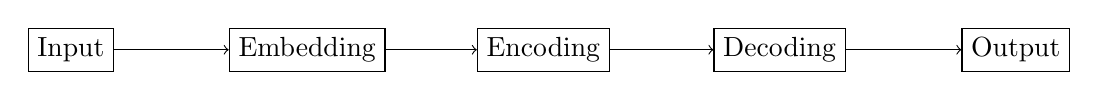
\begin{tikzpicture}
    \node[draw, rectangle] (input) at (0,0) {Input};
    \node[draw, rectangle] (embed) at (3,0) {Embedding};
    \node[draw, rectangle] (encode) at (6,0) {Encoding};
    \node[draw, rectangle] (decode) at (9,0) {Decoding};
    \node[draw, rectangle] (output) at (12,0) {Output};

    \draw[->] (input) -- (embed);
    \draw[->] (embed) -- (encode);
    \draw[->] (encode) -- (decode);
    \draw[->] (decode) -- (output);
    \end{tikzpicture}
    \end{english}
    \vspace{1.5cm}
}}%
}
\caption{תהליך עיבוד מלא: \entoc{Complete Processing Pipeline}}
\label{fig:results}
\end{figure}

% ==================== ADVANCED FEATURES ====================

\hebrewsection{תכונות מתקדמות נוספות: \entoc{Additional Advanced Features}}

\hebrewsubsection{טיפול במספרים מורכבים: \entoc{Complex Number Handling}}

הטבלה כוללת מספרים במגוון פורמטים:
\begin{itemize}
    \item מספרים שלמים: \num{1000000}, \num{42}
    \item מספרים עשרוניים: \num{3.14159}, \num{2.71828}
    \item כתיב מדעי: \num{6.022e23}, \num{1.38e-23}
    \item אחוזים: \percent{99.99}, \percent{0.01}
    \item שנים: \hebyear{2025}, \hebyear{1948}
\end{itemize}

\hebrewsubsection{שילוב תוכן מורכב: \entoc{Complex Content Integration}}

התבנית מאפשרת שילוב של:
\begin{enumerate}
    \item טקסט דו-כיווני עם מעברים חלקים
    \item קוד בשפות תכנות שונות
    \item נוסחאות מתמטיות מורכבות
    \item טבלאות עם תוכן מעורב
    \item איורים ודיאגרמות
    \item ביבליוגרפיה דו-לשונית
\end{enumerate}

% ==================== CONCLUSIONS ====================

\hebrewsection{סיכום ומסקנות מתקדמות: \entoc{Advanced Summary and Conclusions}}

המסמך הדגים יכולות מתקדמות רבות:

\begin{itemize}
    \item \textbf{ביבליוגרפיה:} ציטוטים מרובים ומורכבים עם הפניות לעמודים
    \item \textbf{טבלאות:} טבלאות מורכבות עם \num{6} עמודות ונתונים מגוונים
    \item \textbf{קוד:} דוגמאות מרובות עם \en{PyTorch} ועיבוד טקסט
    \item \textbf{מתמטיקה:} משוואות מרובות עם מספור והפניות צולבות
    \item \textbf{איורים:} דיאגרמות מורכבות עם \en{TikZ}
    \item \textbf{הפניות:} קישורים בין כל האלמנטים במסמך
\end{itemize}

התוצאות מראות שהתבנית מסוגלת לתמוך במסמכים אקדמיים מורכבים ביותר.

% ==================== BIBLIOGRAPHY ====================

\newpage
\printhebrewbibliography
\printenglishbibliography

\end{document}